\documentclass{article}
\title{Nechyba Ch.14 竞争性市场均衡}
\author{Dawei Wang}
\date{\today}
\usepackage{ctex}
\usepackage{amsmath}
\usepackage{amssymb}
\usepackage{graphicx} %插入图片的宏包
\usepackage{float} %设置图片浮动位置的宏包
\usepackage{subfigure} %插入多图时用子图显示的宏包
\begin{document}
	\maketitle
如果一个市场(或行业)中的所有企业都足够小,以至于它们不能单独地操控并影响经济环境,那么这样一个市场(或行业)就被认为是“竞争性”的。均衡市场价格在竞争性行业中起重要作用,这一均衡是一个“去中心化的市场均衡”,意指这一均衡不通过中央计划,而只是通过不同个体分散的决策实现。另一方面,生产是由利己主义和市场价格的形成所知道的。

\section{均衡:组合需求与供给曲线}

假设每个经济人都相对于行业或整个经济都很“小”,以至于没有哪一个可以仅通过自己的力量去改变均衡的结果。那么相应地,对于经济人来说,简单地将世界视为给定,并在其中作出他能作出地最好的决策才是理性的行为,尽管均衡是由所有个体的最优化决策共同决定的,经济环境也由此形成。

\subsection{短期中的均衡}
导出短期中一个具体行业的供需曲线是很容易的,这仅仅是将个体最优化问题所得出的所有需求曲线和供给曲线加总起来即可。

\hspace*{\fill}

个体需求曲线的加总得到了短期市场需求曲线。

个体供给曲线加总得到了短期市场供给曲线(short-run market supply curve)$ S^M $。但注意“供给曲线”加总推导市场供给曲线的做法只适用于短期。


\hspace{\fill}

两曲线的交点表示出市场均衡价格$ p^* $和均衡产出$ X_1^* $。如果市场价格超过这一均衡价格,$ x_1 $的供给量会超过需求量,生产者的库存越来越多,那么他们都会各自降价来出卖他们的商品以求改善情况,反之反是。
$ p^* $成为均衡价格的原因在于,当价格不等于$ p^* $时,每个生产者都有一种自然的把价格向$ p^* $调整的趋势,意即只有当价格等于$ p^* $时,才没有哪一个有动机去调整他的价格。

市场通过均衡价格向消费者和生产者发出信号,用一种分散化的方式协调他们的行为,并且在某些情况下这一方式是“有效的”。

产品市场中的需求曲线来自所有消费模型中商品束的消费者;劳动市场的需求曲线来自于雇佣劳动力的生产者;资本市场中的需求曲线来自于厂商的资本需求。

\subsection{长期均衡中的市场(行业)}

厂商除了在长期中的投入要素种类比短期中更多之外,厂商在长期中有进入或退出行业的机会,这就意味着虽然在短期行业里的厂商的数目是固定的(尽管有些厂商会关闭),但长期中厂商数量是可变的,因为长期中厂商会随着市场环境的变化进入或者退出行业。

规范地说,我们将厂商的“长期”定义为它可以调整那些短期中的固定要素投入水平的时期,对于一个行业来说,“长期”是指厂商可以进入或者退出行业的时期。唯一不一样的是有些厂商固定自己资本投入的时间比其他厂商更短一些,并且只有当足够多的厂商可以进入和退出行业时才能成为一个行业的“长期”。

厂商的短期供给曲线是(短期)MC曲线在(短期)AC之上的部分,然而在长期中,厂商需要收回它所有的经济成本,那么此时也就包括了短期中那些固定投入的支出以及其他固定成本(如许可证费);因此一个厂商如果可以收回成本,那么它会进入某个行业并赚取一些利润,如果不能则它会退出该行业。因此,长期中如果价格低于长期AC曲线,厂商会退出所在行业。

\begin{figure}[H] %H为当前位置,!htb为忽略美学标准,htbp为浮动图形
	\centering %图片居中
	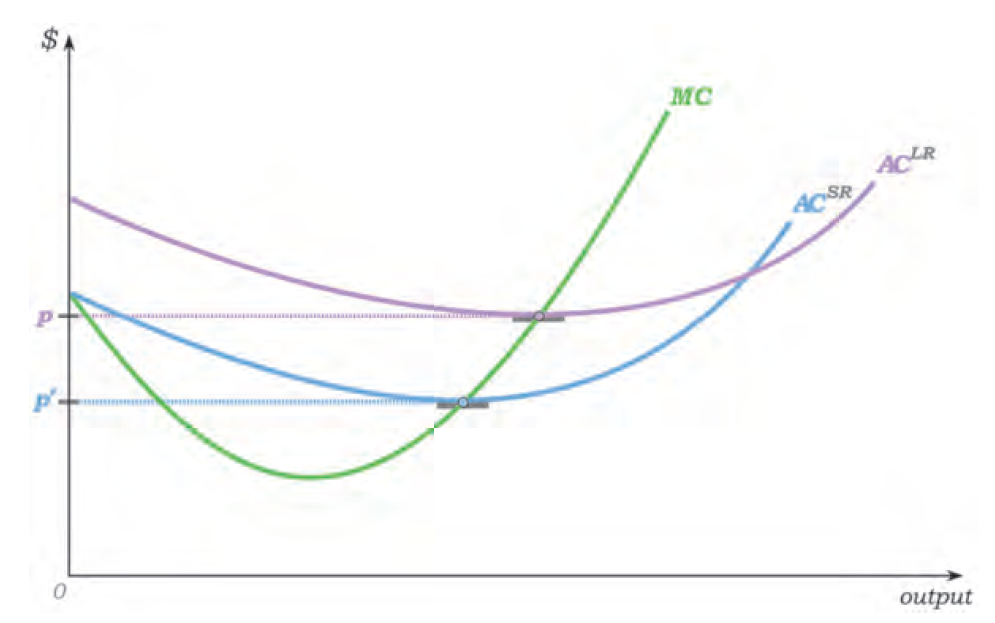
\includegraphics[width=1\textwidth]{14_1} %插入图片,[]中设置图片大小,{}中是图片文件名
	\caption{Shutting Down versus Exiting an Industry} %最终文档中希望显示的图片标题
	\label{Fig.main2} %用于文内引用的标签
\end{figure}

\hspace*{\fill}

当所有生产者同质时的长期均衡价格
\begin{figure}[H] %H为当前位置,!htb为忽略美学标准,htbp为浮动图形
	\centering %图片居中
	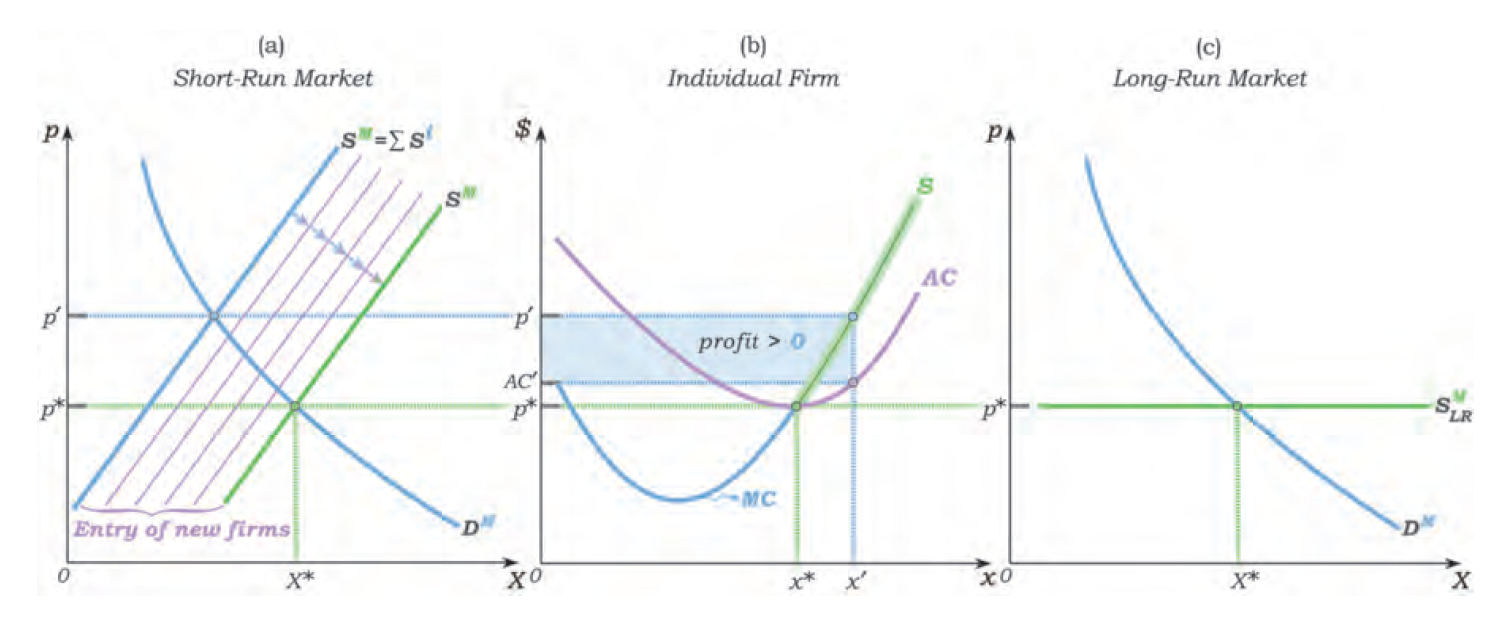
\includegraphics[width=1\textwidth]{14_2} %插入图片,[]中设置图片大小,{}中是图片文件名
	\caption{Moving from Short-Run to Long-Run Equilibrium} %最终文档中希望显示的图片标题
	\label{Fig.main3} %用于文内引用的标签
\end{figure}

长期市场供给曲线是水平的并且处于AC的最低点。当长期中厂商可以进入和退出行业时,市场会以位于AC曲线最低点$ p^* $的价格提供所需任意的产品数量。这就意味着长期市场(或行业)供给曲线并不是通过加总单个厂商的供给曲线而来,而是通过厂商的进入和退出决策影响价格,使得它们的长期利润为零得到的;即价格最终会落在单个厂商长期AC
曲线的最低点。

\hspace*{\fill}

对于产品市场的某一种商品,厂商的进入和退出使得长期和短期均衡有所不同,但一般来讲,同样的事情对于劳动力市场均衡来说并不适用,至少当某个行业相对于整个经济比较小时是不成立的。当某个行业相对于整个经济很小时,影响该行业的因素往往并不会影响整个劳动力市场。因此,单个行业中的厂商的进入和退出不能被认为是移动劳动力曲线的重要原因。

如果某类劳动力的工资变化足够显著,以致引发工人选择再教育或者新一批工人会选择过去工人不同程度的教育,那么进入和退出就会影响劳动力供给曲线。

\hspace*{\fill}

生产者不同时的长期市场供给曲线

我们推导水平的行业长期供给曲线时,明确架设了生产者同质,为了使这一结论(市场长期供给曲线是水平的)成立,事实上只需要假设所有厂商的技术水平使它们的AC曲线最低点在相同的价格上即可,而不用管曲线其他部分的形状如何。

现在假设不同的生产者所拥有的技术显著不同,那么就有可能在一个给定的产品价格下,有些生产者可以获利但有些不能。这也就影响到当市场环境变化时哪些会进入哪些会退出,也影响着长期市场供给曲线的形状。

\begin{figure}[H] %H为当前位置,!htb为忽略美学标准,htbp为浮动图形
	\centering %图片居中
	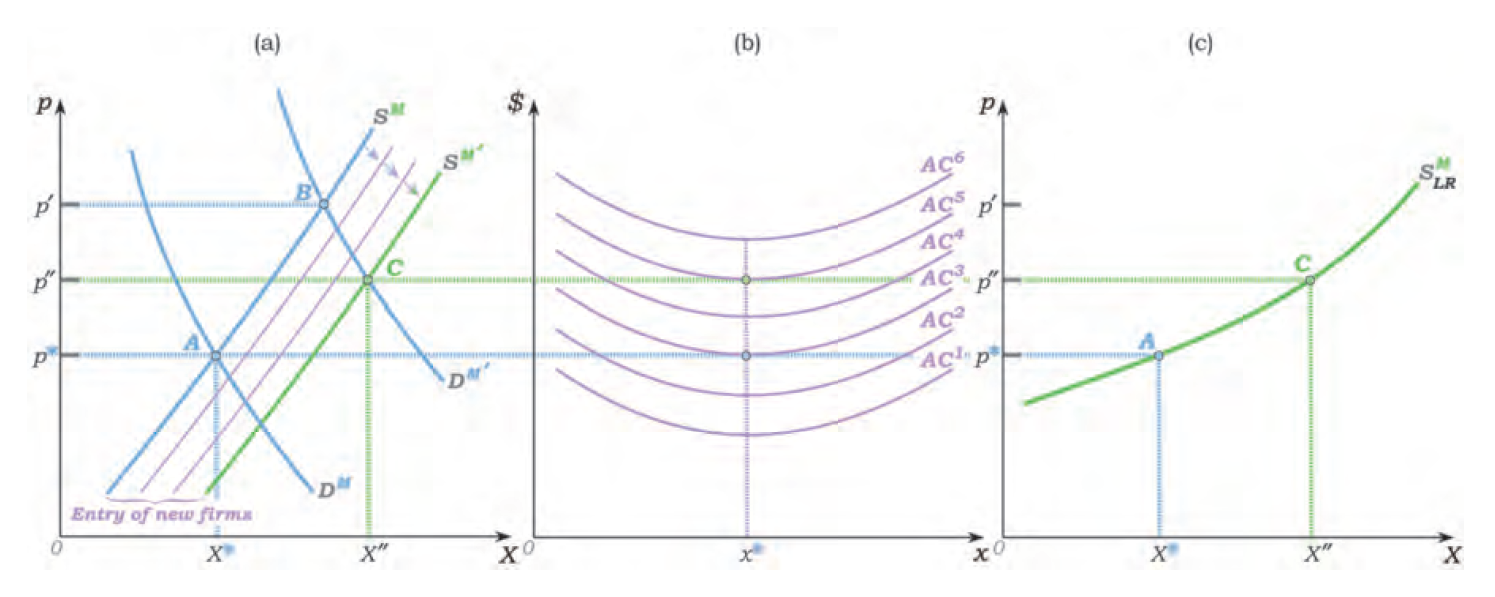
\includegraphics[width=1\textwidth]{14_3} %插入图片,[]中设置图片大小,{}中是图片文件名
	\caption{Long-Run Market Supply when Firms Differ} %最终文档中希望显示的图片标题
	\label{Fig.main4} %用于文内引用的标签
\end{figure}

总的来看,图(a)中的市场需求曲线从$ D^M $移动到$ D^{M'} $使得短期中均衡从A移动到B,长期中均衡落在C,短期中价格从$ p^* $移至$ p' $,长期落在$ p'' $。

长期市场供给曲线不是由单个厂商的供给曲线决定的,而仅仅由厂商AC曲线的最低点的分布决定的。像这样具有向上倾斜的(长期)市场供给曲线的行业被称为成本递增行业。

理论上来讲,但厂商成本随着行业扩张而下降时,长期市场供给曲线也有可能是向下倾斜的。比如,当某行业的扩张导致专供该行业的投入要素的市场竞争加剧时,所有厂商的成本都会下降,就有可能出现这种情况。这样的行业称为成本下降行业。

\hspace*{\fill}

厂商进入与退出行业的过程知直到边际厂商(在长期中)赚取零利润为止。“边际厂商”指的是行业中成本最高的生产者。

\subsection{改变条件与改变均衡}

在竞争性行业中,“经济条件的变化”可以在某种程度上表示为需求和供给的变化,那么短期或长期均衡就会变化。

对于生产者来说,条件的改变可能源自:(1)可变成本的变化,如工资;(2)短期中固定投入相关的固定支出的改变;(3)只有退出行业才能避免的固定成本的改变。

对于消费者来说:消费者的偏好的改变或者市场中新产品的出现可能会使市场需求曲线移动。

\subsubsection{长期均衡中的短期均衡}

假设我们的行业现在处于一个长期均衡状态,这意味着边际厂商赚取(长期的)零利润,因此它们在长期AC曲线的最低点位置的价格水平生产。

注意,行业中的每个厂商在短期中都赚取正利润。这是因为短期经济成本完全包含在了短期平均成本曲线之中。并且短期平均成本曲线的最低点低于长期AC曲线的最低点。短期供给曲线是MC的一部分,因此它随着(短期)边际成本的变化而移动。

\subsubsection{改变长期固定成本}

假设长期固定成本提高,由于其不属于短期平均或边际成本的一部分,因此不影响短期决策(短期AC、MC)均不变。

对于长期而言,长期固定成本增加使得(长期)AC曲线向上移动,但是长期供给曲线(MC)不变。

\begin{figure}[H] %H为当前位置,!htb为忽略美学标准,htbp为浮动图形
	\centering %图片居中
	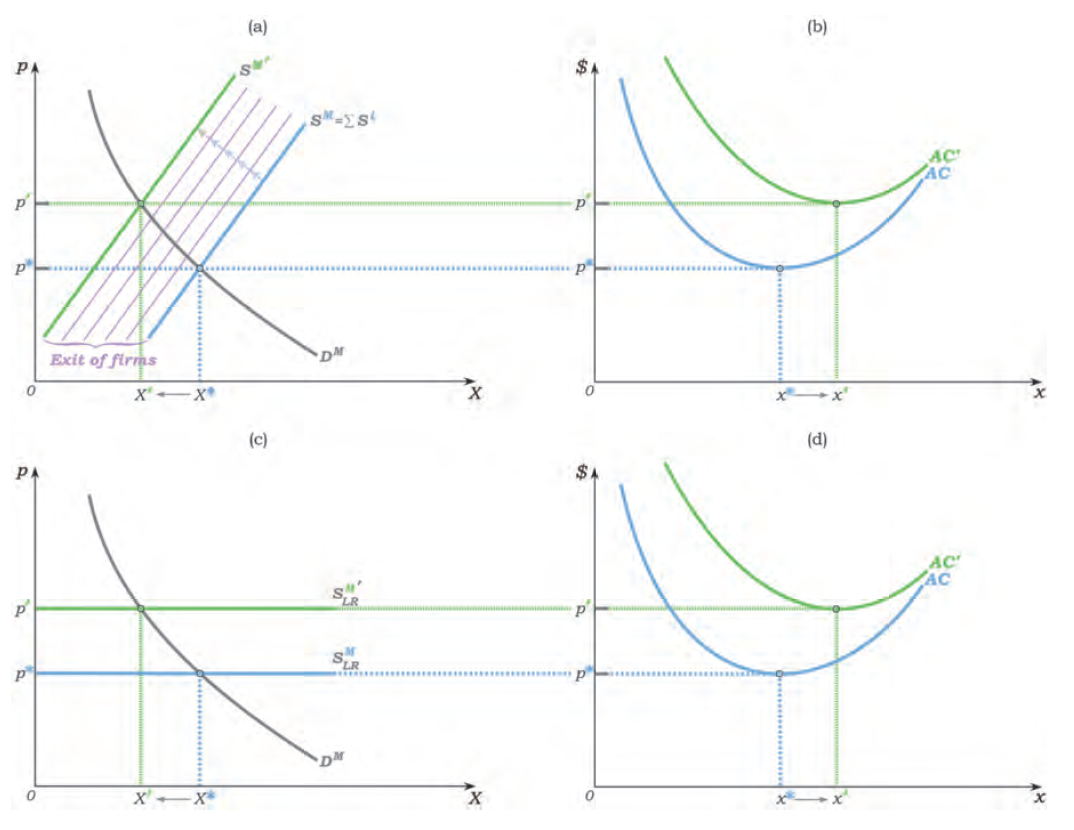
\includegraphics[width=1\textwidth]{14_4} %插入图片,[]中设置图片大小,{}中是图片文件名
	\caption{An Increase in a Long-Run Fixed Cost} %最终文档中希望显示的图片标题
	\label{Fig.main5} %用于文内引用的标签
\end{figure}

尽管厂商短期利润不变,但是长期利润现在变为负值,这就使得一些厂商退出该行业,从而使得短期市场供给曲线$ S^M $向内移动。$ S^M $向内移动抬高了市场价格,并且持续会有厂商退出,直到新均衡价格达到图(b)中$ AC' $曲线的最低点。只有当市场价格上升到$ p' $,行业内的厂商才能再次赚取零利润,也就没有厂商有动机进出该行业了。

总之,留下来的厂商个体生产更多,但是市场总产出下降。

图(c)和图(d)描述了厂商同质时的情形

\subsubsection{改变短期固定投入价格}

考虑资本价格上升(资本是短期固定但长期可变的投入)。

资本价格上升不影响短期决策。由于资本价格的上升相当于长期可变成本的增加,因此每个厂商长期MC曲线都会上移,因此资本价格上升后厂商的AC最低点与之前相比是在左还是在右不确定(不确定留存的单个厂商是否会多生产)。这取决于生产技术的特点。而且由于在资本价格上升的一瞬间并不处于长期均衡,此时的短期MC曲线并不穿过长期AC的最低点,但是经过调整后(增加k)的MC曲线(使其处于长期均衡)仍穿过长期AC的最低点。

总之,资本价格的上升使得部分厂商退出该行业,厂商的退出导致市场供给减少,均衡价格上升,直至所有厂商盈亏平衡为止。市场的长期供给曲线上升。行业产出下降,留存的厂商个体产出上升或者下降取决于其生产技术的特点。

\subsubsection{改变可变成本}

假设可变成本提高。

\begin{figure}[H] %H为当前位置,!htb为忽略美学标准,htbp为浮动图形
	\centering %图片居中
	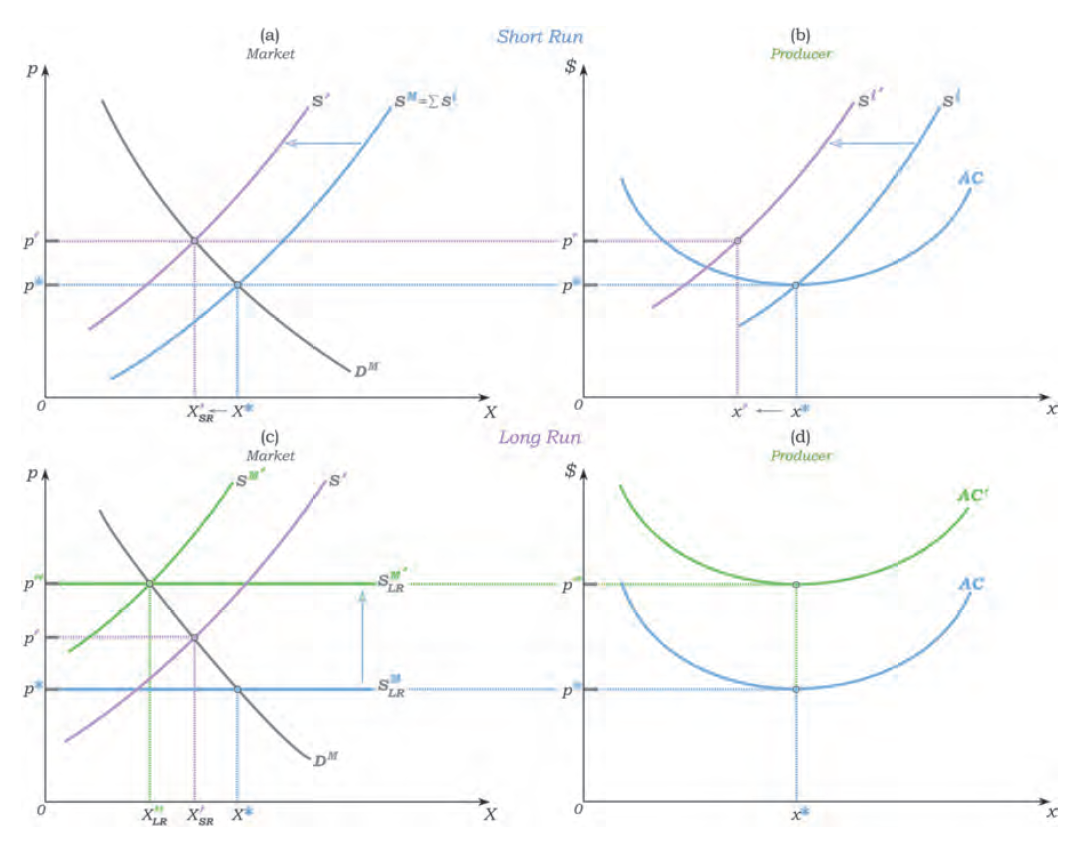
\includegraphics[width=1\textwidth]{14_5} %插入图片,[]中设置图片大小,{}中是图片文件名
	\caption{An Increase in the Wage} %最终文档中希望显示的图片标题
	\label{Fig.main6} %用于文内引用的标签
\end{figure}

假设厂商同质,厂商短期供给曲线左移引致短期市场供给曲线左移,短期产品价格上升。由于厂商同质,所有厂商继续生产,但市场总产量会下降。因此短期中价格会上升至足够多(到$ p' $)以保证短期利润大于零。

若假设厂商不同质,则一些厂商比另一些厂商成本低,一旦高成本厂商不能赚取非负的利润,它们将在短期内关闭。

长期中,价格必须调整至新的$ AC' $的最低点,意味着图(c)中的长期市场供给曲线从开始的水平线$ S^M_{LR} $上升至新的$ S^M_{LR'} $,价格变为$ p'' $。

单个厂商新的$ AC' $的最低点的产量相较于$ AC $的最低点的产量不明确,取决于厂商生产技术的特点。理论上可以变大、变小或者不变。相应地,市场内厂商数量可能减少、不变或增加。

\subsubsection{改变需求}

市场需求的变化可能来自于消费者口味的变化(组成市场需求曲线的个人需求曲线发生了变化),或者来自于相关市场新产品的引入,也可能是由于新的消费者群体进入市场。像这样的需求变化是不会影响到厂商的成本曲线的,意味着我们不需要对厂商的成本曲线做任何改变。

\begin{figure}[H] %H为当前位置,!htb为忽略美学标准,htbp为浮动图形
	\centering %图片居中
	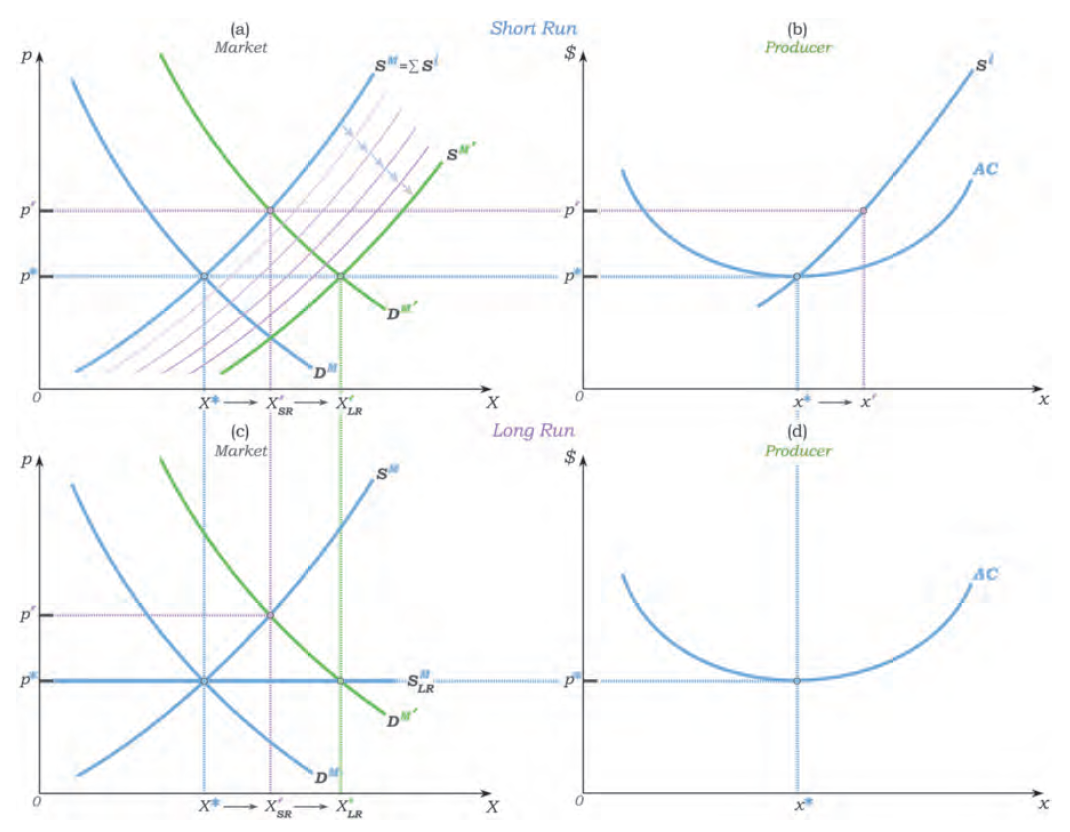
\includegraphics[width=1\textwidth]{14_6} %插入图片,[]中设置图片大小,{}中是图片文件名
	\caption{An Increase in Market Demand} %最终文档中希望显示的图片标题
	\label{Fig.main7} %用于文内引用的标签
\end{figure}

在图(a)和图(c)中,在短期中市场产出上升到$ X'_{SR} $,而最终在长期达到一个更高的产出水平$ X'_{LR} $。在图(b)中,我们进一步看到一开始行业中每个厂商都增加了自己的产量,但图(d)说明了每个厂商最终会生产与需求增加之前相同的产量。因此也就说明了,整个市场产量的增加仅仅是因为新厂商的进入,从而扩大了整个行业的规模。

\subsubsection{影响单个厂商的变动与影响整个行业的变动}
有时候可能只是行业中的某个厂商发生某种变化。这针对厂商特有变化的分析会变得相当简单,因为每个厂商对于竞争行业来说都是足够下的,所以单个厂商的行为变化不会影响行业的短期和长期均衡。

\begin{figure}[H] %H为当前位置,!htb为忽略美学标准,htbp为浮动图形
	\centering %图片居中
	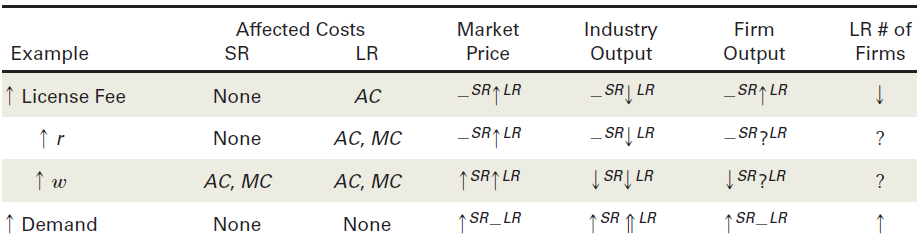
\includegraphics[width=1\textwidth]{14_7} %插入图片,[]中设置图片大小,{}中是图片文件名
	\caption{The Impact of Changing Conditions of Firms and Industries (assuming
		Identical Firms)} %最终文档中希望显示的图片标题
	\label{Fig.main8} %用于文内引用的标签
\end{figure}

\hspace*{\fill}

上述均衡是基于这样的假设,即个体——生产者和消费者——相对于经济是“小的”,从而不能独自影响他们所处的经济环境。

竞争均衡中值得关注的点在于它描述了一种“自发的秩序”,我们说“秩序”是一种机制,它通过市场价格发出信号,使得千百万的个体行为人得知他们该如何与市场中的其他人合作。我们说“自发”是指秩序的形成无需任何人规划。

实际上,在一定条件下,可以证明这些自发的秩序利用从社会可得的稀缺资源,实现了最大化总体收益。




\end{document}